\subsection{Motivación}
\subsubsection{Stakeholder}
El punto de vista de Stakeholder le permite al analista modelar las partes interesadas, los conductores internos y externos para el cambio, y las evaluaciones (en términos de fortalezas, debilidades, oportunidades y amenazas) de estos controladores. Además, los vínculos con la inicial (alto nivel) objetivos que abordan estas preocupaciones y las evaluaciones pueden ser descritas. Estos objetivos constituyen a la base para el proceso de ingeniería de requisitos, incluyendo el refinamiento objetivo, análisis de la contribución y el conflicto, y la derivación de los requisitos que dan cuenta de los objetivos. \citeW{ArchiMat55:online} \vspace{\baselineskip}

En el caso de estudio, vemos los objetivos principales, con sus implicados y sus valoraciones de MusicApp. Se pueden ver sus puntos fuertes y a mejorar.

\newpage
\paragraph{Modelo}:
\begin{figure}[h!]
	\centering
	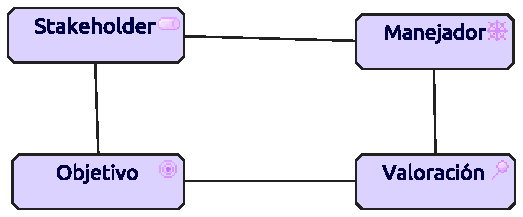
\includegraphics[width=0.6\linewidth]{Desarrollo/ArquitecturaEmpresarial/Motivacion/imgs/stakeholderMetamodelo.pdf}
	\caption{Modelo: stakeholder}
\end{figure}
\paragraph{Caso de Estudio}:

\begin{figure}[h!]
	\centering
	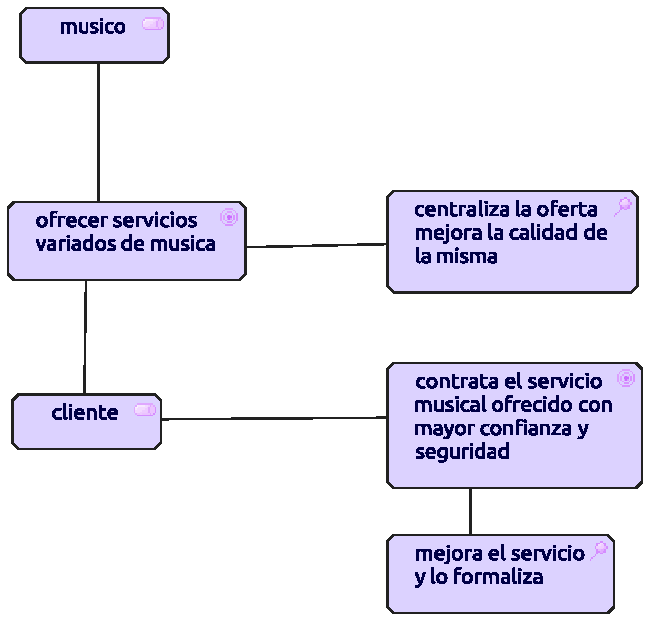
\includegraphics[width=0.7\linewidth]{Desarrollo/ArquitecturaEmpresarial/Motivacion/imgs/stakeholder.pdf}
	\caption{Caso de estudio: stakeholder}
	\label{fig:comportamiento}
\end{figure}

\newpage

\subsubsection{Realización de Objetivos}
El punto de vista de Realización de Objetivos permite a un diseñador modelar el refinamiento de los objetivos (alto nivel) en objetivos más concretos, y el refinamiento de objetivos concretos en requisitos o condiciones que describen las propiedades que son necesarias para alcanzar los objetivos. El refinamiento de las metas en sub-objetivos se modela utilizando la relación de agregación. El refinamiento de las metas en los requisitos se modela utilizando la relación realización. \citeW{ArchiMat55:online} \vspace{\baselineskip}

A continuación se modelan los objetivos de alto nivel para la aplicación MusicApp, estos permitirán el refinamiento en objetivos más concretos dentro de los siguientes modelos.

\paragraph{Modelo}:
\begin{figure}[h!]
	\centering
	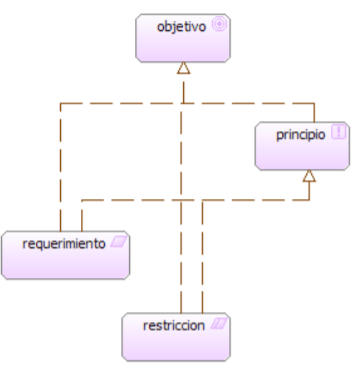
\includegraphics[width=0.6\linewidth]{Desarrollo/ArquitecturaEmpresarial/Motivacion/imgs/realizacionObjMetamodelo.PNG}
	\caption{Modelo: Realización de Objetivos}
\end{figure}
\paragraph{Caso de Estudio}:

\begin{figure}[h!]
	\centering
	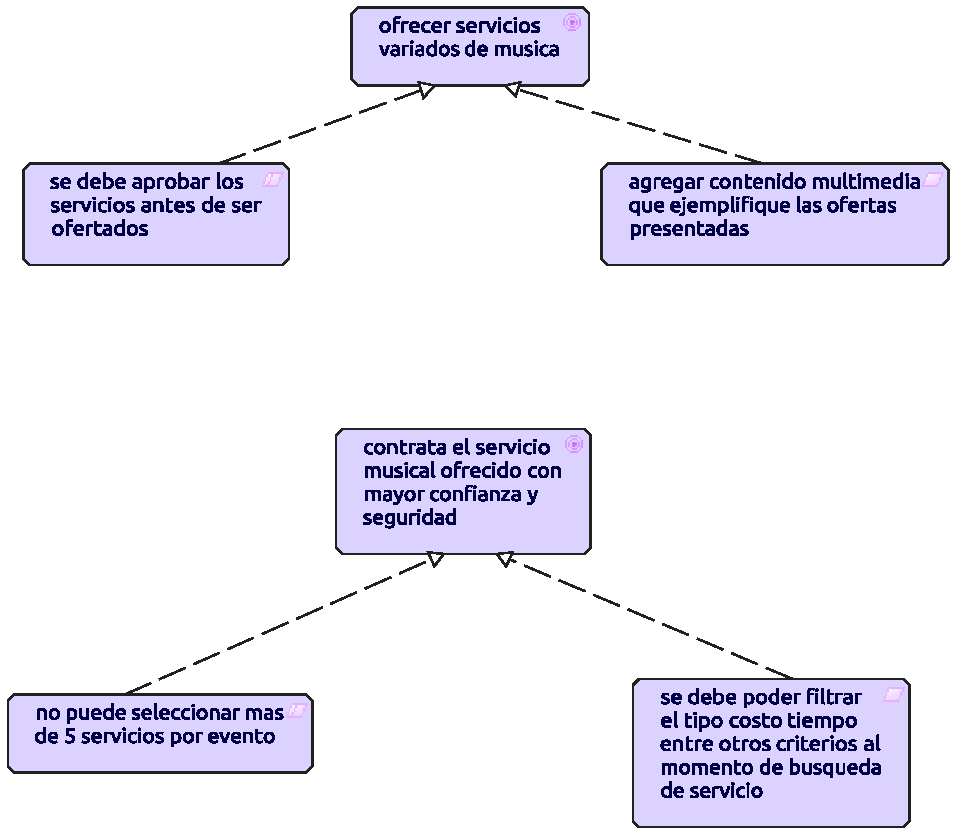
\includegraphics[width=\linewidth]{Desarrollo/ArquitecturaEmpresarial/Motivacion/imgs/realizacionObj.pdf}
	\caption{Caso de estudio: Realización de Objetivos}
	\label{fig:comportamiento}
\end{figure}

\newpage

\subsubsection{Contribución}
El punto de vista de contribución le permite a un diseñador o analista modelar las relaciones de influencia entre los objetivos y requisitos. Los puntos de vista resultantes se pueden utilizar para analizar el impacto que tienen sobre los objetivos entre sí o para detectar conflictos entre los objetivos de las partes interesadas.
 \citeW{ArchiMat55:online} \vspace{\baselineskip}

El siguiente punto de vista muestra las relaciones entre objetivos y requisitos de forma general, permite enfocarse en un valor clave del producto el cual es la agilidad en búsqueda y contratación de músicos

\paragraph{Modelo}:
\begin{figure}[h!]
	\centering
	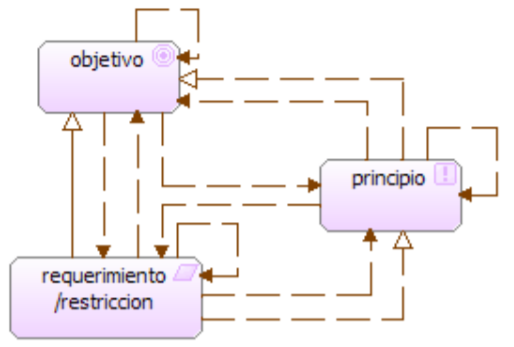
\includegraphics[width=0.6\linewidth]{Desarrollo/ArquitecturaEmpresarial/Motivacion/imgs/ContribucionMetamodelo.PNG}
	\caption{Modelo: Contribución}
\end{figure}
\newpage
\paragraph{Caso de Estudio}:
\begin{figure}[h!]
	\centering
	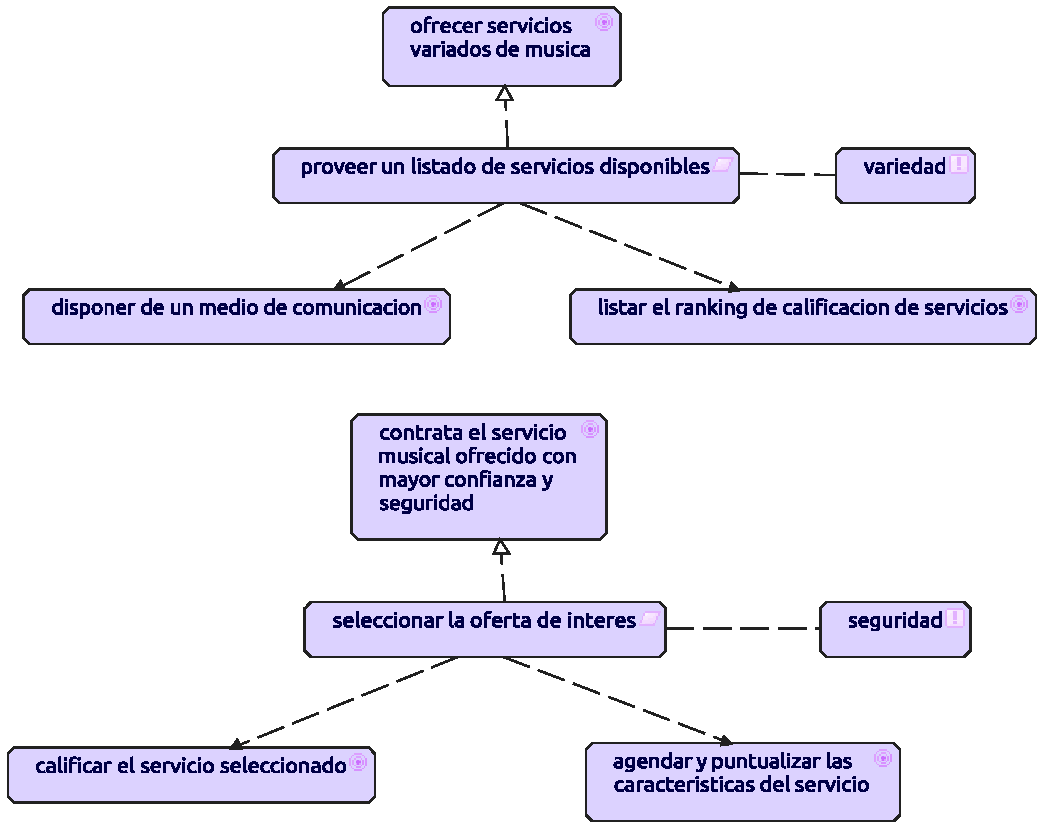
\includegraphics[width=\linewidth]{Desarrollo/ArquitecturaEmpresarial/Motivacion/imgs/Contribucion.pdf}
	\caption{Caso de estudio: Contribución}
	\label{fig:comportamiento}
\end{figure}

\newpage


\subsubsection{Principios}
El punto de vista de contribución le permite a un diseñador o analista modelar las relaciones de influencia entre los objetivos y requisitos. Los puntos de vista resultantes se pueden utilizar para analizar el impacto que tienen sobre los objetivos entre sí o para detectar conflictos entre los objetivos de las partes interesadas.
 \citeW{ArchiMat55:online} \vspace{\baselineskip}

El siguiente punto de vista muestra las relaciones entre objetivos y requisitos de forma general, permite enfocarse en un valor clave del producto el cual es la agilidad en búsqueda y contratación de músicos

\paragraph{Modelo}:
\begin{figure}[h!]
	\centering
	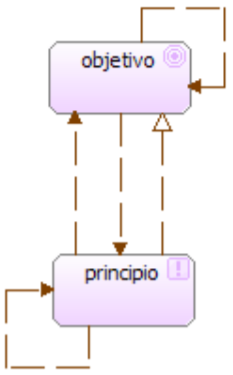
\includegraphics[width=0.4\linewidth]{Desarrollo/ArquitecturaEmpresarial/Motivacion/imgs/PrincipiosMetamodelo.PNG}
	\caption{Modelo: Principios}
\end{figure}
\newpage
\paragraph{Caso de Estudio}:
\begin{figure}[h!]
	\centering
	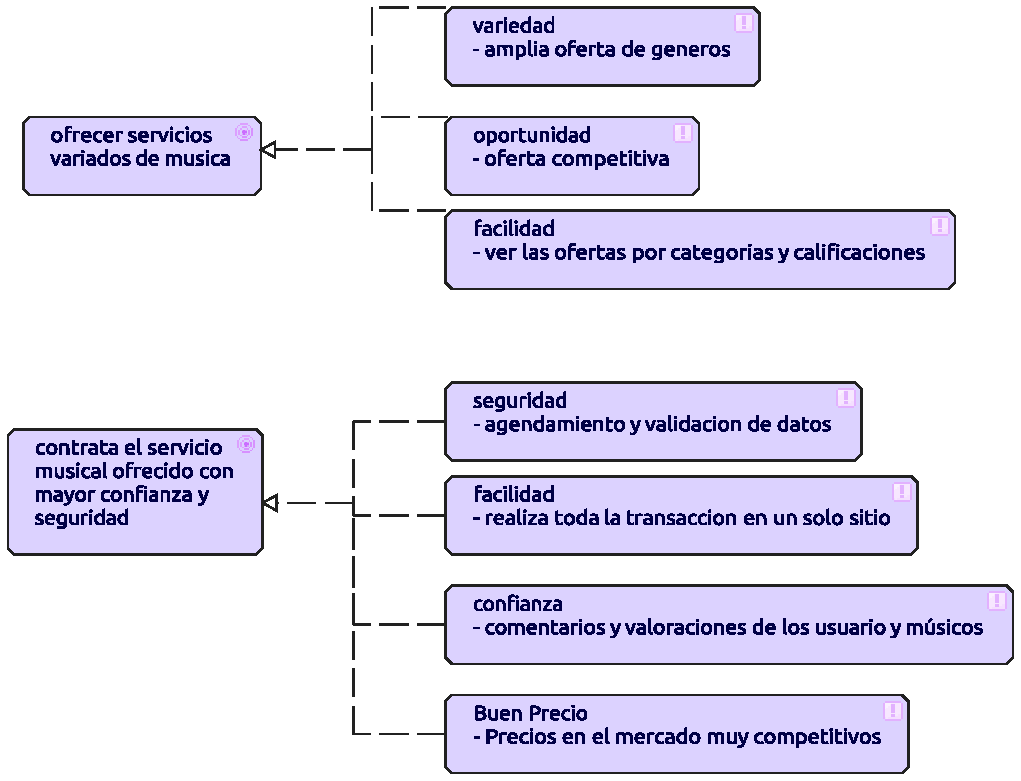
\includegraphics[width=\linewidth]{Desarrollo/ArquitecturaEmpresarial/Motivacion/imgs/Principios.pdf}
	\caption{Caso de estudio: Principios}
	\label{fig:comportamiento}
\end{figure}

\newpage

\subsubsection{Realización de Requerimientos}
El Punto de vista de Realización de Requerimientos permite al diseñador modelar la realización de los requisitos por parte de los elementos básicos, tales como agentes de negocios, servicios de oficina, los procesos de negocios, servicios de aplicaciones, componentes de la aplicación, etc. \citeW{ArchiMat55:online} \vspace{\baselineskip}

El siguiente punto de vista permite modelar los objetivos claves para la creación de la aplicación MusicApp el cual representa el objetivo general del proyecto

\paragraph{Modelo}:
\begin{figure}[h!]
	\centering
	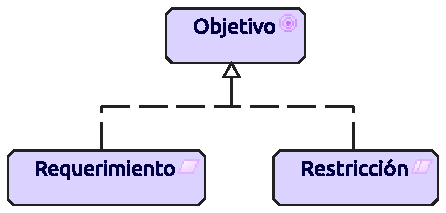
\includegraphics[width=0.8\linewidth]{Desarrollo/ArquitecturaEmpresarial/Motivacion/imgs/RealizacionMetamodelo.pdf}
	\caption{Modelo: Realización de Requerimientos}
\end{figure}
\newpage
\paragraph{Caso de Estudio}:
\begin{figure}[h!]
	\centering
	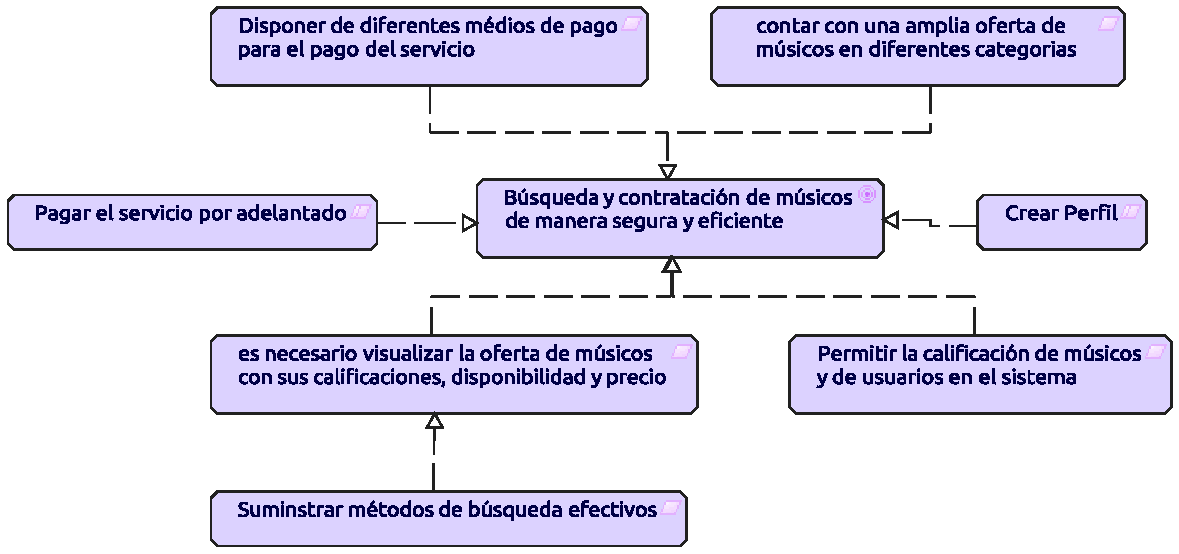
\includegraphics[width=\linewidth]{Desarrollo/ArquitecturaEmpresarial/Motivacion/imgs/Realizacion.pdf}
	\caption{Caso de estudio: Realización de Requerimientos}
	\label{fig:comportamiento}
\end{figure}

\newpage

\subsubsection{Motivación}
El Punto de vista de Motivación permite al diseñador o analista modelar el aspecto de motivación, sin centrarse en determinados elementos dentro de este aspecto. Por ejemplo, este punto de vista se puede utilizar para presentar una visión completa o parcial del aspecto de la motivación por los interesados relacionados, sus objetivos principales, los principios que se aplican, y los principales requerimientos de servicios, procesos, aplicaciones y objetos. \citeW{ArchiMat55:online} \vspace{\baselineskip}

El siguiente modelo representa las motivaciones para el proyecto, describe a modo general los objetivos y la dependencia de riesgo con las actividades de investigación e implementación del desarrollo del prototipo.

\paragraph{Modelo}:
\begin{figure}[h!]
	\centering
	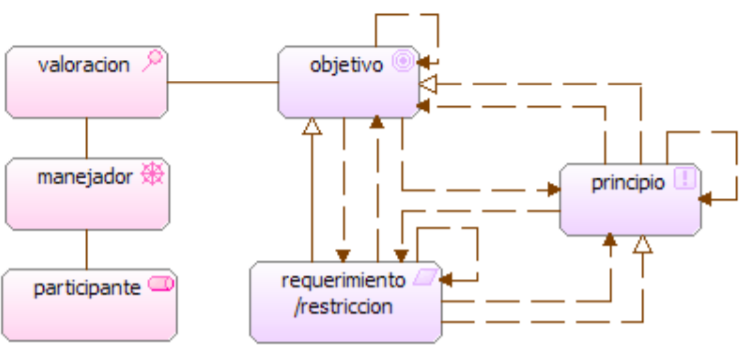
\includegraphics[width=0.8\linewidth]{Desarrollo/ArquitecturaEmpresarial/Motivacion/imgs/MotivacionMetamodelo.PNG}
	\caption{Modelo:  Motivación}
\end{figure}
\newpage
\paragraph{Caso de Estudio}:
\begin{figure}[h!]
	\centering
	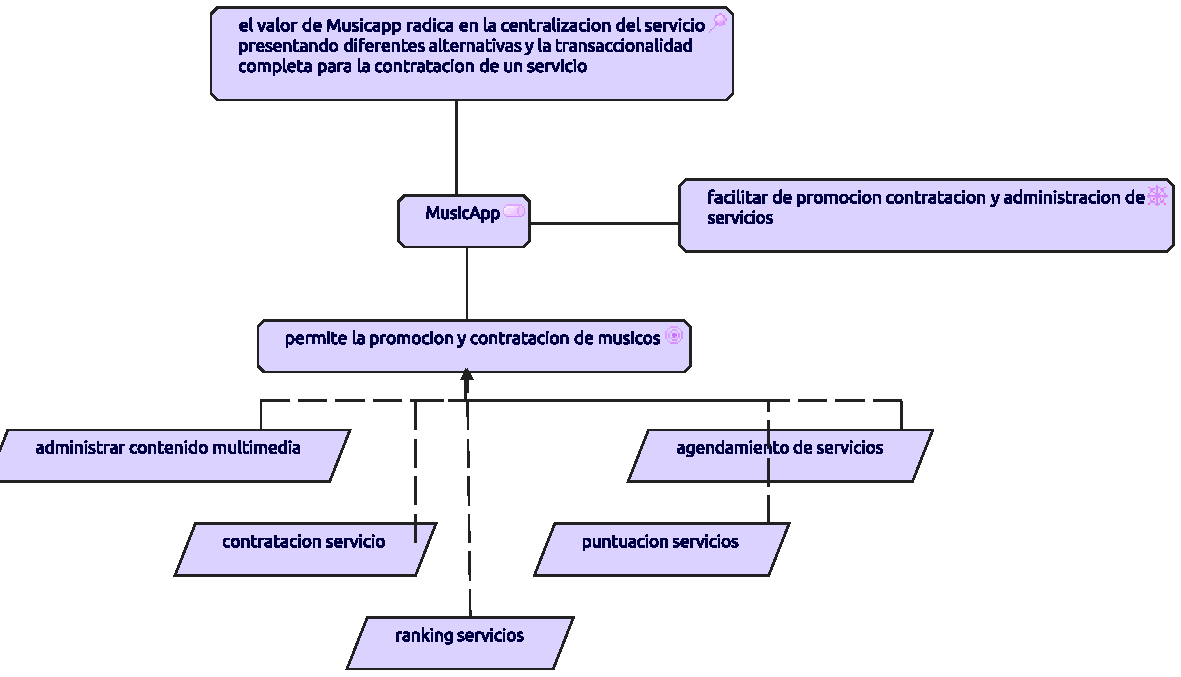
\includegraphics[width=\linewidth]{Desarrollo/ArquitecturaEmpresarial/Motivacion/imgs/Motivacion.pdf}
	\caption{Caso de estudio: Motivación}
	\label{fig:comportamiento}
\end{figure}

\newpage

